% !TeX spellcheck = fr_FR
\thispagestyle{noheader}
\chapter*{Résumé} % No (numbered) toc entry with *

\tikz[remember picture,overlay] \node[shift={(4.165cm,-1.955cm)}]
	at (current page.north west)
	{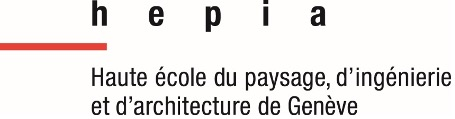
\includegraphics[height=1.29cm]{template/images/title/hepia_logo}};
	\tikz[remember picture,overlay] \node[shift={(-4.238cm,-1.97cm)}]
	at (current page.north east)
	{
\includegraphics[height=1.29cm]{template/images/title/hes-so_geneve_logo}};

\addcontentsline{toc}{chapter}{Résumé} % Adding toc entry
\thispagestyle{noheader}

\begin{spacing}{0.956}
\vspace{0.5cm}

%% CONTENT STARTS HERE
Lorsqu'un utilisateur doit s'authentifier auprès d'un service, il doit fournir un mot de passe préalablement défini. 
Pour des raisons de sécurité, le système stocke ce mot de passe en le passant par une fonction de hachage. 
Ainsi, lors de l'authentification, le système compare le hash du mot de passe entré par l'utilisateur avec le hash stocké pour vérifier son identité. 
Une fonction de hachage qui est souvent utilisé pour le stockage de mots de passe est le Bcrypt, qui a comme particularité d'être assez lente, rendant les mots de passe assez résistante aux attaques par bruteforce. 
Ce rapport a pour but de détailler la mise en oeuvre d'un système visant à attaquer les mots de passe protégés par l'algorithme bcrypt en utilisant un \gls{fpga}. 
L'objectif principal est de créer une solution extensible et plus performante que les approches traditionnelles basées sur \gls{gpu}. 
Le système repose sur plusieurs cœurs de calcul parallèles sur le \gls{fpga} pour générer les hashs bcrypt. 
Ce projet présente deux solutions distinctes pour l'implémentation d'une attaque par bruteforce. 
La première solution génère les mots de passe directement sur le \gls{fpga}, accompagnée d'une interface \gls{uart} qui permet à l'utilisateur d'interagir avec le système. 
La seconde solution, encore en développement, repose sur l'utilisation de l'interface \gls{pcie} pour permettre des transferts de données rapides, rendant ainsi possible une attaque par dictionnaire. 
Après l'implémentation, des mesures ont été effectuées pour évaluer les performances et l'utilisation des ressources sur le \gls{fpga}. 
Bien que la solution basée sur l'interface \gls{pcie} ne soit pas encore entièrement opérationnelle, les résultats obtenus jusqu'à présent ouvrent la voie à des optimisations et des améliorations futures.

\vfill
\begin{center}
	{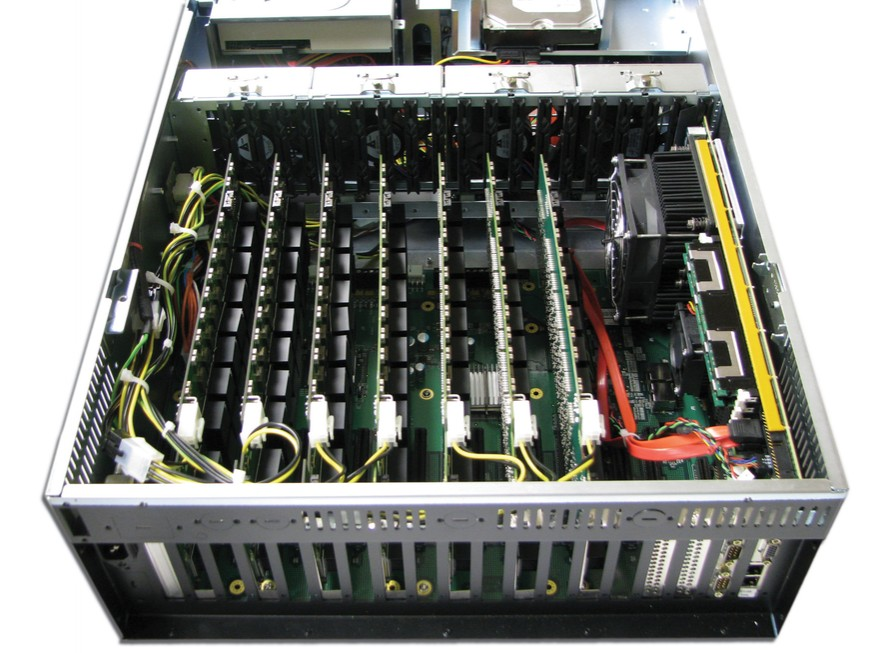
\includegraphics[width=0.4\linewidth]{figures/fpga_cluster}}\\*
\vfill
%% CONTENT ENDS HERE

{
%%%%%%%%%%%%%%%%%%%%%%%%%%%%%%%%%%%%%%%%%%%%%%%%%%%%%%%%%%%%%%%%%%%%%%%%%%%%%%%%
%%%%%%%%%%%%%%%%%%%%%%%%%% DO NOT MODIFY THE TABLE BELOW %%%%%%%%%%%%%%%%%%%%%%%
%%%%%%%%%%%%%%%%%%%%%%%%%%%%%%%%%%%%%%%%%%%%%%%%%%%%%%%%%%%%%%%%%%%%%%%%%%%%%%%%
	\begin{tabular*}{16cm}{p{7.59cm} p{7.58cm}}
		\small Candidat-e:					&	\small Professeur-e(s) responsable(s):\\*[10pt]
		\small\textbf{\textsc{\Author}}		&	\small\textbf{\textsc{\Professor}}\\*[10pt]
		\footnotesize  Filière d’études : ISC	&	\footnotesize  \textbf{En collaboration avec:} ELCA Security\\*[10pt]
		\footnotesize  {} & \footnotesize  Travail de bachelor soumis à une convention de stage en entreprise: \Convention\\*[20pt]
		\footnotesize  {} & \footnotesize  Travail soumis à un contrat de confidentialité: \Confidentiel\\*[10pt]
	\end{tabular*}\\*[1.9cm]
}
	
	%\textit{Attention : Tout l’énoncé doit tenir sur une seule page}
\end{center}
\end{spacing}
